\chapter{Weight Diagrams}
\label{ch-weight-diagrams}
This chapter is based on Refs. \cite{eli-daw-book}
and \cite{lich-book}.

In this chapter, we will study irreps of semi-simple Lie algebras,
paying special attention to $\ger{su}(2)$ and $\ger{su}(3)$.
Suppose $\ger{g}$ is the Lie algebra of a group $G$.
Note that an irrep of $G$ always gives an irrep of $\ger{g}$,
but an irrep of $\ger{g}$ might not give an irrep of $G$.
Suppose groups $G_1$ and $G_2$ with different global topology both have Lie algebra $\ger{g}$.
Some irreps of $\ger{g}$ might lead to irreps of $G_1$ but not of $G_2$.
For example, $SO(3)$ and $SU(2)$
have the same Lie algebra
$\ger{su}(2)$. $\ger{su}(2)$ has irreps with integral
and half integral spin. But only
the ones with integral spin are irreps of $SO(3)$.
Luckily, for $SU(n)$, which is the group that most cooncerns us
in this chapter, all irreps of $\ger{su}(n)$
are irreps of $SU(n)$ too. 

In Chapter \ref{ch-dynkin},
we classified semi-simple Lie algebras
in terms of their Dynkin diagrams. The Dynkin diagram of a Lie algebra $\ger{g}$ describes its set of
root vectors. An irrep of $\ger{g}$
is described by a set of weight vectors.
Both {\bf root vectors} and {\bf weight vectors}  satisfy an eigenvalue equation, namely 
\beq
\begin{array}{ll}
\text{root }\valp:&
\overbrace{[\vec{H}, E_{\vec{\alp}}]}^
{[\vec{H},\;\cdot\;]E_{\vec{\alp}}}
= \vec{\alp} E_{\vec{\alp}}
\\
\text{weight $\vec{m}$:}&
\vec{H}\ket{j, \vec{m}}= \vec{m}\ket{j, \vec{m}}
\end{array}
\eeq

$\vec{\alp}, \vec{m}\in\RR^r$
where $r$ is the rank of the Lie algebra.

$\ket{1}, \ket{2}, \ldots, \ket{n}\in \RR^n$ and
$H_i, E_{\vec{\alp}}\in \RR^{n\times n}$  where $n$ is
the dimension of the fundamental rep of the Lie algebra $\ger{su}(n)$

$\ket{j, \vec{m}}\in \CC^d$ where $d$ is the dimension of the irrep.

The set of weight vectors of an irrep of a Lie algebra will be called the
{\bf Weight Diagram (WD)} of the irrep.

\begin{figure}[h!]
\centering
\includegraphics[width=2.5in]
{weight-diagrams/weight-roots-relation.png}
\caption{Relationship between 2 weights $\vec{m}$ and $\vec{m}'$.}
\label{fig-weight-roots-relation}
\end{figure}

\begin{claim}
If 

\beq
\vec{H}\ket{\vec{m}}
=\vec{m}\ket{\vec{m}}
\eeq
then
\beq
\vec{H}E_{\vec{\alp}}\ket{\vec{m}}
=(\vec{m}+\vec{\alp})E_{\vec{\alp}}\ket{\vec{m}}
\eeq
\end{claim}
\proof
\beq
[\vec{H}, E_{\vec{\alp}}]=\vec{\alp}E_{\vec{\alp}}
\eeq
so
\beqa
\vec{H}E_{\vec{\alp}}\ket{\vec{m}}
&=&
E_{\vec{\alp}}\vec{H}\ket{\vec{m}} + \vec{\alp}E_{\vec{\alp}}\ket{\vec{m}}
\\&=&
(\vec{m}+\vec{\alp})E_{\vec{\alp}}\ket{\vec{m}}
\eeqa
\qed

\begin{claim} See Fig.\ref{fig-weight-roots-relation}.
For any weight $\vec{m}$ and
root $\vec{\alp}$,
if $k$ is an integer and

\beq k = -\;\frac{2\vec{m}\cdot \vec{\alp}}{\vec{\alp}\cdot\vec{\alp}}
\eeq
then

\beq
\vec{m}'=\vec{m} + k\vec{\alp}
\eeq
is a weight
with the same eigenvalue multiplicity as $\vec{m}$.
\end{claim}
\proof
\qed


\section{$SU(2)$ Weight Diagrams}

In this section, we describe 
the WDs for $SU(2)$. These
follow from the 
theory of angular momentum
in Quantum Mechanics.

Define
\beq
\ket{1}=\begin{pmatrix}
1
\\
0
\end{pmatrix}
,\quad
\ket{2}=\begin{pmatrix}
0
\\
1
\end{pmatrix}
\eeq

\beq
\sqrt{2}E_{12}=J_+=\ket{1}\bra{2},\quad
\sqrt{2}E_{-12}=E_{21}=J_- =\ket{2}\bra{1}
\eeq

\beq
J_z=\frac{1}{2}\left(
\ket{1}\bra{1}
-\ket{2}\bra{2}\right)
\eeq
Then

\beq
\begin{array}{ll}
\bcen
\xymatrix{
&J_z\ar[dl]_{-J_-}
\ar[dr]^{J_+}
\\
J_-&&J_+\ar[ll]^{2J_z}
}
\ecen
&
\left\{
\begin{array}{l}
[J_+, J_-]=2J_z
\\
{[J_z, J_+]=J_+}
\\
{[J_z, J_-]=-J_-}
\end{array}\right.
\end{array}
\eeq



The WD for irrep $j$, where\footnote{Whenever possible, we will follow  the convention of denoting operators by upper case letters 
and their eigenvalues
by the same letter in lower case.
For example, 
the eigenvalues of $J,J_z$ 
will be denoted by $j, j_z$.
}
\beq
J=j\in \left\{0, \frac{1}{2}, 1, \frac{3}{2}, \ldots\right\}
\eeq
has weights $m$, where

\beq
J_z=j_z=m=\{-j, -j+1, \ldots, j-1, j\}
\eeq

$\ket{j,m}$ is the basis vector of irrep $j$ with weight $m$.

\section{$SU(3)$ Weight Diagrams}

In this section, we describe 
the WDs for $SU(3)$. These
occur in particle
physics, 
when describing 
particles by their
quark constituents.

Define

\beq
\ket{1}=\begin{pmatrix}
1
\\
0
\\
0
\end{pmatrix}
,\quad
\ket{2}=\begin{pmatrix}
0
\\
1
\\
0
\end{pmatrix}
,\quad
\ket{3}=\begin{pmatrix}
0
\\
0
\\
1
\end{pmatrix}
\eeq

\beq
\sqrt{3}E_{12}=T_+=\ket{1}\bra{2},\quad
\sqrt{3}E_{-12}=E_{21}=T_- =\ket{2}\bra{1}
\eeq

\beq
\sqrt{3}E_{23}=U_+ = \ket{2}\bra{3},\quad
\sqrt{3}E_{-23}=E_{32} = U_- = \ket{3}\bra{2}
\eeq

\beq
\sqrt{3}E_{31}=V_+ = \ket{3}\bra{1},\quad
\sqrt{3}E_{-31}=E_{13}=V_- = \ket{1}\bra{3}
\eeq

\beq
T_z = \frac{1}{2}
\left(
\ket{1}\bra{1}
-\ket{2}\bra{2}\right),
\quad
U_z = \frac{1}{2}
\left(
\ket{2}\bra{2}
-\ket{3}\bra{3}\right)
,\quad
V_z = \frac{1}{2}
\left(
\ket{3}\bra{3}
-\ket{1}\bra{1}\right)
\eeq


\beq
\sqrt{\frac{3}{2}}H_1=T_z,
\quad
\sqrt{2}H_2=Y=
\frac{2}{3}
\left(
U_z-V_z
\right)
\eeq

{\bf isospin} $T_z\in \ZZ/2= 0, \pm\frac{1}{2}, \pm 1, \pm\frac{3}{2}, \pm 2, \ldots$

{\bf hypercharge} $Y\in \ZZ/3$


$H_1\in 
\frac{1}{\sqrt{6}}\ZZ$

$H_2\in \frac{1}{3\sqrt{2}}\ZZ$


\begin{figure}[h!]
\centering
\includegraphics[width=2.4in]
{weight-diagrams/123-vecs.png}
\caption{$\ket{1}, \ket{2}, \ket{3}$ 
vectors, and operators that act on them. $E_{-ij}=E_{ji}$ is in opposite direction 
as $E_{ij}$ for $i\ne j$ and $i,j=1,2,3$.}
\label{fig-123-vecs}
\end{figure}
Fig.\ref{fig-123-vecs}
illustrates the states $\ket{1}, \ket{2}, \ket{3}$, and operators $E_{ij}$ that act on them. 


We can derive
the weights of the 
fundamental rep
of $\ger{su}(3)$ as follows.

\renewcommand{\arraystretch}{1.5}
\beq
\begin{pmatrix}
\sqrt{\frac{3}{2}}H_1
\\
\sqrt{2}H_2
\end{pmatrix}
\ket{1}
=
\begin{pmatrix}
T_z
\\
Y
\end{pmatrix}
\ket{1}
=
\begin{pmatrix}
\frac{1}{2}
\\
\frac{1}{3}
\end{pmatrix}
\ket{1}
=
\vec{m}(1)\ket{1}
\eeq

\beq
\begin{pmatrix}
\sqrt{\frac{3}{2}}H_1
\\
\sqrt{2}H_2
\end{pmatrix}
\ket{2}
=
\begin{pmatrix}
T_z
\\
Y
\end{pmatrix}
\ket{2}
=
\begin{pmatrix}
-\frac{1}{2}
\\
\frac{1}{3}
\end{pmatrix}
\ket{2}
=
\vec{m}(2)\ket{2}
\eeq

\beq
\begin{pmatrix}
\sqrt{\frac{3}{2}}H_1
\\
\sqrt{2}H_2
\end{pmatrix}
\ket{3}
=
\begin{pmatrix}
T_z
\\
Y
\end{pmatrix}
\ket{3}
=
\begin{pmatrix}
0
\\
-\frac{2}{3}
\end{pmatrix}
\ket{3}
=
\vec{m}(3)\ket{3}
\eeq
\renewcommand{\arraystretch}{1}



\begin{figure}[h!]
\centering
\includegraphics[width=3.5in]
{weight-diagrams/weights-fundamental.png}
\caption{The roots vectors of $\ger{su}(3)$ in green and the weight vectors  of the fundamental rep in red.}
\label{fig-weights-fundamental}
\end{figure}

Fig.\ref{fig-weights-fundamental}
shows 
the root vectors for $\ger{su}(3)$ (derived in Chapter \ref{ch-dynkin}) and the
weight vectors  of the fundamental rep
of $\ger{su}(3)$ (just derived).
As expected, the difference between
any two weight vectors, is $k$ times a root vector.



\begin{figure}[h!]
\centering
\includegraphics[width=3.5in]
{weight-diagrams/tuv-plus.png}
\caption{
Each of the six root
vectors of $\ger{su}(3)$
is associated with a raising operator $T_+, U_+, V_+$
or a lowering operator
$T_-, U_-, V_-$.}
\label{fig-tuv-plus}
\end{figure}

As shown in Fig.\ref{fig-tuv-plus},
each of the six root
vectors of $\ger{su}(3)$
is associated with a raising operator $T_+, U_+, V_+$
or a lowering operator
$T_-, U_-, V_-$.
In $\ger{su}(2)$
$J_+$ raises the $J_z=j_z=m$ of a quantum state by
$1/2$ and $J_-$
lowers it by a $1/2$.
$T_\pm, U_\pm, V_\pm$ change $T_z,U_z, V_z$ analogously.

\subsection{Examples}

In this section, we give examples of
$SU(3)$ WDs.

There is a
one-to-one map
between the the irreps of  $\ger{su}(3)$ and the WDs
of $\ger{su}(3)$.

The weights on the {\bf boundary of WD} are called {\bf dominant weights
}

In a WD, nondegenerate weights are
represented by a single dot.
$k$-fold degenerate weights (i.e., eigenvalues with {\bf {\bf multiplicity}} $k$) are represented by a dot with $k-1$ rings.

WD are labelled either by

\begin{itemize}
\item the dimension $d_{rep}$ of the irrep, with extra labels in case there are multiple irreps with the same dimension, 

\item the
$(\lam, \mu)$ WD-boundary dimensions. See Fig.\ref{fig-rep15}
\end{itemize}

One can show that


\beq
d_{rep}= \frac{1}{2}(\lam+1)(\mu+1)(\lam +\mu +2)
\label{eq-drep}
\eeq

For example, see Fig.\ref{fig-3-3star}. $\ger{su}(3)$ has 2 fundamental irreps, $\ul{3}$ and $\ul{3}^*$. Both are 3 dimensional. $(\lam,\mu)=(1,0)$ for $\ul{3}$, 
and $(\lam,\mu)=(0,1)$ for $\ul{3}^*$.
The formula Eq.(\ref{eq-drep}) for $d_{rep}$ gives 3 for both.

See the following figures for examples of WDs of $\ger{su}(3)$.

\begin{itemize}
\item Fig.\ref{fig-3-3star}
shows $\ul{3}$ and $\ul{3}^*$

\item Fig.\ref{fig-rep10}
shows $\ul{10}$ (decuplet)

\item Fig.\ref{fig-rep8}
shows $\ul{8}$ (octet)

\item Fig.\ref{fig-rep15}
shows $\ul{15}$

\end{itemize}


\begin{figure}[h!]
\centering
\includegraphics[width=2.9in]
{weight-diagrams/rep3.png}
\includegraphics[width=2.9in]
{weight-diagrams/rep3star.png}
\caption{WDs for the two fundamental irreps of $\ger{su}(3)$, $\ul{3}$ and $\ul{3}^*$. $(\lam,\mu)=(1,0)$ for $\ul{3}$, 
and $(\lam,\mu)=(0,1)$ for $\ul{3}^*$.}
\label{fig-3-3star}
\end{figure}


\begin{figure}[h!]
\centering
\includegraphics[width=3.5in]
{weight-diagrams/rep10.png}
\caption{WD for the $\ger{su}(3)$ irrep $\ul{10}$. $(\lam,\mu)=(3,0)$.}
\label{fig-rep10}
\end{figure}

\begin{figure}[h!]
\centering
\includegraphics[width=3.5in]
{weight-diagrams/rep8.png}
\caption{WD for the $\ger{su}(3)$ irrep $\ul{8}$. $(\lam,\mu)=(1,1)$.}
\label{fig-rep8}
\end{figure}

\begin{figure}[h!]
\centering
\includegraphics[width=3.5in]
{weight-diagrams/rep15.png}
\caption{WD for the $\ger{su}(3)$ irrep $\ul{15}$. $(\lam,\mu)=(2,1)$.}
\label{fig-rep15}
\end{figure}

\hrule
{\bf An aside about hypercharge}

Several different quantum numbers are called hypercharge in particle physics. For example, in the
Gell-mann-Nishijima relation
\beq Q= T_z + \frac{1}{2}Y'\eeq
hyperchage= $Y'\in \ZZ$, isospin= $T_z\in \ZZ/2$, so charge= $Q\in\ZZ/2$. For example,
for nucleons, 
\beq \text{proton (p)}: \quad T_z=\frac{1}{2},\quad Y'=1\implies Q=1\eeq
\beq\text{neutron (n)}: \quad T_z=-\;\frac{1}{2},\quad Y'=1\implies Q=0\eeq
As a mnemonic, remember that a nucleon has 3 quarks with $Y=1/3$,
and $Y'$ for the nucleon is the sum of $Y$ for each quark. $Y=1/3$ for up or down quarks, and $Y=-2/3$ for the strange quark. $u,d$ constitute an $SU(2)$ doublet and $s$ an $SU(2)$ singlet.

\section{Relation between WD and Semi-Standard Young Tableaux}

Young Diagrams (YD) and Young Tableaux (YT) are 
discussed in Chapter \ref{ch-young-tableau}

Given a YD, its SYT/SSYT (Standard or Semi-Standard YT) 
satisfies


\begin{itemize}
\item Rows strictly/weakly increasing
\item Columns strictly increasing
\item Entries in $\{1,2,\dots, n\}$.
$n=3$ for $SU(3)$
\end{itemize}
Thus, SYT/SSYT disallow/allow repetitions along a row.

SYT are used, for example, to label the irreps of $S_n$.
Hence, there is a 1-1 relation between Young Symmetrizer operators
and SYT. 


SSYT are used below to label the basis weight vectors of an irrep of $\ger{su}(n)$.
There is a 1-1 relationship between YD and WD,
and a 1-1 relationship between the SSYT of a YD and the 
weights of the corresponding WD.
Degenerate weights have different SSYT.

To summarize,

SYTs \xymatrix{\ar[r]_{\text{1 to 1}}&} Young operators, SSYTs \xymatrix{\ar[r]_{\text{1 to 1}}&} weights of WD



To calculate
the isospin, hypercharge
$(t_z, y)$
of a SSYT, 
use the follwing equation

\beq
(t_z,y)=
\sum_{\text{boxes}}
\left\{
\begin{array}{ll}
(\frac{1}{2},\frac{1}{3}), & \text{for each 1 box}\\
(-\frac{1}{2},\frac{1}{3}), & \text{for each 2 box}\\
(0,-\frac{2}{3}), & \text{for each 3 box}
\end{array}
\right.
\eeq
Equivalently,
if $n_i$ is the number
of $i=1,2,3$ boxes
in the SSYT, then

\beq
t_z=
\frac{1}{2}(n_1-n_2)
\eeq

\beq 
y=\frac{1}{3}(n_1 + n_2 - 2 n_3)
\eeq
\hrule
SU(3) octet example. 


An octet ($\ul{8}$, (1,1), Fig.\ref{fig-rep8})
has the YD

$$
\ydiagram{2,1}
$$
Let 

\beq
\caly = S_{12}A_{13}= [1+(12)][1-(13)]
\eeq
Then

\beqa\ket{\psi}=
\caly\ket{a}\ket{b}\ket{c}
&=&
S_{12}\left(
\ket{a}\ket{b}\ket{c}-\ket{c}\ket{b}\ket{a}
\right)
\\&=&
[\ket{a}\ket{b}\ket{c} + \ket{b}\ket{a}\ket{c}]
-[\ket{c}\ket{b}\ket{a}+\ket{b}\ket{c}\ket{a}]
\eeqa

The following
table gives 
the SSYT, its $(t_z, y)$
content, and its
wavefunction,
for each weight of an $SU(3)$ octet.  This table's information is conveyed pictorially
in Fig.\ref{fig-rep8-with-yt}.

\begin{enumerate}

\item
\beq 
\begin{array}{l|l|l}
\begin{ytableau}
1 & 1\\
2
\end{ytableau}
&
(t_z,y)=\left(+\tfrac12,1\right)
&\ket{\psi} \text{ with } abc\rarrow u_1
u_1 u_2
\end{array}
\eeq 

\item

\beq 
\begin{array}{l|l|l}
\begin{ytableau}
1 & 2\\
2
\end{ytableau}
&
(t_z,y)=\left(-\tfrac12,1\right)
& \ket{\psi} \text{ with } abc\rarrow u_1 u_2 u_2
\end{array}
\eeq 


\item
\beq
\begin{array}{l|l|l}
\begin{ytableau}
1 & 1\\
3
\end{ytableau}
&
(t_z,y)=(+1,0)
&
\ket{\psi} \text{ with } abc\rarrow u_1 u_1 u_3
\end{array}
\eeq 

\item
\beq
\begin{array}{l|l|l}
\begin{ytableau}
1 & 2\\
3
\end{ytableau}
&
(t_z,y)=(0,0)
&
\ket{\psi} \text{ with } abc\rarrow u_1 u_2 u_3
\end{array}
\eeq 

\item

\beq 
\begin{array}{l|l|l}
\begin{ytableau}
2 & 2\\
3
\end{ytableau}
&
(t_z,y)=(-1,0)
&
\ket{\psi} \text{ with } abc\rarrow u_2 u_2 u_3
\end{array}
\eeq 


\item 

\beq 
\begin{array}{l|l|l}
\begin{ytableau}
1 & 3\\
2
\end{ytableau}
&
(t_z,y)=(0,0)
&\ket{\psi} \text{ with } abc\rarrow u_1 u_3 u_2
\end{array}
\eeq 


\item

\beq 
\begin{array}{l|l|l}
\begin{ytableau}
1 & 3\\
3
\end{ytableau}
&
(t_z,y)=\left(+\tfrac12,-1\right)
&
\ket{\psi} \text{ with } abc\rarrow u_1 u_3 u_3
\end{array}
\eeq 

\item

\beq 
\begin{array}{l|l|l}
\begin{ytableau}
2 & 3\\
3
\end{ytableau}
&
(t_z,y)=\left(-\tfrac12,-1\right)
& \ket{\psi} \text{ with } abc\rarrow u_2 u_3 u_3
\end{array}
\eeq 

\end{enumerate}

\begin{figure}[h!]
\centering
\includegraphics[width=3.5in]
{weight-diagrams/rep8-with-yt.png}
\caption{WD for the $SU(3)$ octet with the SSYT
for each weight.}
\label{fig-rep8-with-yt}
\end{figure}


